% Exact E:x²/16+y²/12=1, H:x²-y²/3=1; P=(2,3).
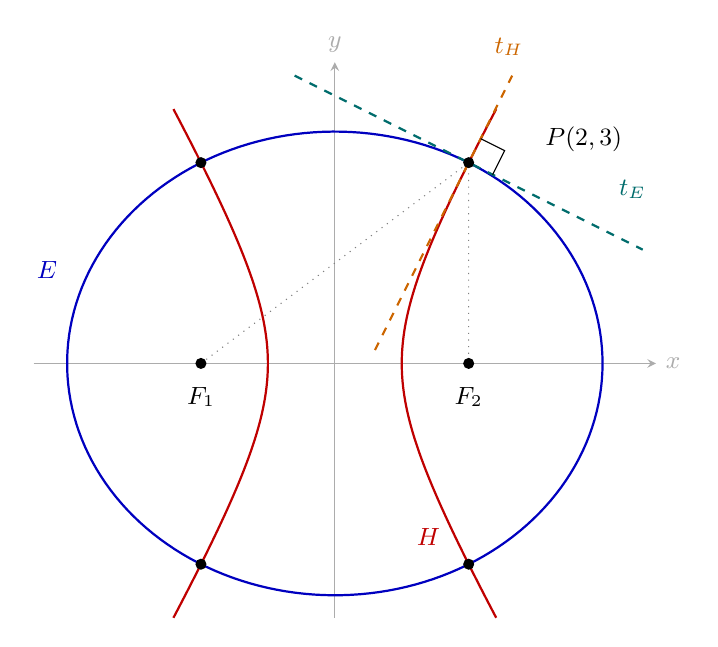
\begin{tikzpicture}[x=.85cm,y=.85cm,>=stealth,font=\small]
\draw[gray!65,->] (-4.5,0)--(4.8,0) node[right] {$x$};
\draw[gray!65,->] (0,-3.8)--(0,4.5) node[above] {$y$};
\draw[blue!75!black,thick,domain=0:360,samples=180,variable=\t]
 plot ({4*cos(\t)},{sqrt(12)*sin(\t)});
\foreach \s in {-1,1} {
\draw[red!75!black,thick,domain=-3.8:3.8,samples=100,variable=\t]
 plot ({\s*sqrt(1+\t*\t/3)},\t);}
\draw[teal!85!black,thick,dashed] (-.6,4.3)--(4.6,1.7);
\draw[orange!80!black,thick,dashed] (.6,.2)--(2.65,4.3);
\draw[gray,dotted] (-2,0)--(2,3)--(2,0);
\foreach \s in {-1,1} {\foreach \t in {-1,1}
 {\fill ({2*\s},{3*\t}) circle (2pt);}}
\fill (-2,0) circle (2pt) node[below=5pt] {$F_1$};
\fill (2,0) circle (2pt) node[below=5pt] {$F_2$};
\node[anchor=west] at (3,3.35) {$P(2,3)$};
\node[teal!85!black,anchor=west] at (4.1,2.6) {$t_E$};
\node[orange!80!black,above] at (2.6,4.45) {$t_H$};
\node[blue!75!black] at (-4.3,1.4) {$E$};
\node[red!75!black] at (1.4,-2.6) {$H$};
\draw (2.358,2.821)--(2.537,3.179)--(2.179,3.358);
\end{tikzpicture}
